% arXiv preprint — extended version of the SPIE Medical Imaging submission.
% v2 (2026-08-31): full prose revision; v1 is preserved as main_v1.tex.
% Editorial revision by Codex, 2026-09-07; original manuscript preserved.
% Build: tectonic main_by_codex.tex
\documentclass[11pt]{article}

\usepackage[letterpaper,margin=1in]{geometry}
\usepackage{amsmath,amssymb}
\usepackage{graphicx}
\usepackage{booktabs}
\usepackage{algorithm}
\usepackage{algpseudocode}
\usepackage{placeins}
\usepackage[font=small,labelfont=bf]{caption}
\usepackage{microtype}
\renewcommand{\topfraction}{0.9}
\renewcommand{\textfraction}{0.05}
\renewcommand{\floatpagefraction}{0.8}
\interfootnotelinepenalty=10000
\usepackage{xcolor}
\definecolor{linkblue}{RGB}{25,60,120}
\usepackage[colorlinks=true,linkcolor=linkblue,citecolor=linkblue,urlcolor=linkblue]{hyperref}

\emergencystretch=1.5em
\renewcommand{\thesection}{\Roman{section}}
\renewcommand{\thesubsection}{\Alph{subsection}}
\makeatletter
\renewcommand{\p@subsection}{\thesection .}
\makeatother

\newcommand{\FDK}{\mathrm{FDK}}
\newcommand{\thetahat}{\hat\theta}
\newcommand{\Pnom}{P_{\mathrm{nom}}}




\begin{document}
\begin{center}{\Large \textbf{Rigid-Motion Correction in Head Cone-Beam CT with a 3D Flow-Matching Prior on a Geometry Bridge\_by\_codex}}\\[10pt]
Sungho Yun and Seungryong Cho\\
Department of Nuclear and Quantum Engineering,\\
Korea Advanced Institute of Science and Technology (KAIST), Daejeon 34141, South Korea\end{center}

\textbf{Abstract}

Blind motion correction in head cone-beam CT (CBCT) requires joint estimation of the
image and per-view rigid poses. We propose a 3D flow-matching prior trained on a geometry
bridge: FDK reconstructions generated from the same volume as the simulated motion
amplitude decreases linearly to zero. The bridge connects the uncorrected reconstruction
to its motion-free FDK counterpart, with an analytic velocity target derived from the
forward projector's geometry derivative. At inference, a predictor-corrector loop
alternates image updates from the frozen prior, motion fitting with a hash-encoded network,
and data-consistency updates. We evaluated the method on simulated projections from 30
held-out CQ500 patients with 10\,mm\,/\,10° peak-to-peak rigid motion. The final
reconstructions achieved 36.66\,dB PSNR and 0.978 SSIM, while mean reprojection error
decreased from 6.12 to 0.28\,mm. Reprojection error was 2.26\,mm for learned autofocus
and 0.84\,mm for JRM-ADM; the proposed reconstructions exceeded JRM-ADM by 7.0\,dB and
0.066 SSIM under the same evaluation protocol. Inference took 9.3 minutes per patient
on an RTX A6000. Replacing the geometry bridge with a pixel-linear path reduced PSNR
by approximately 1.4\,dB, supporting the use of a motion-based training path for joint
image and motion recovery.

\section{I. Introduction}


Cone-beam CT is used for head and neck imaging in image-guided radiotherapy,
interventional suites and point-of-care settings. Head motion during acquisition
violates the static-object assumption of analytic reconstruction, producing streaks and
double contours. A six-degree-of-freedom (6-DoF) rigid pose per projection view provides
a useful model of skull motion. Recovering these poses from the projections alone is
challenging because the image used to estimate the motion is itself corrupted by that
motion. The forward model is linear in the volume but nonlinear in the poses, making
their joint estimation a non-convex problem.

Autofocus methods estimate motion by optimizing an image-quality measure of the
reconstruction. Classical approaches use criteria such as image sharpness[1],
while learned approaches predict voxel-wise visual information fidelity
(VIF)[2] or a scalar quality score[3]. Image-domain methods
instead map corrupted reconstructions directly to corrected images without estimating
the acquisition poses[4]. Autofocus provides efficient motion estimation, but
the pose search depends on how well its quality metric distinguishes residual motion
artifacts from anatomical structure, particularly under severe motion.

Generative image priors offer another way to guide joint recovery, building on
plug-and-play reconstruction[5] and diffusion-based inverse
solvers[6]. JRM-ADM[7] combines a wavelet-domain diffusion
prior (W3DM[17]) with weighted-least-squares image updates and B-spline motion
estimation. Its prior is trained to recover clean volumes from noisy inputs, and the
image and motion updates are incorporated into the diffusion sampling schedule. This
training path is defined by noise corruption; it does not explicitly represent the
image changes caused by reducing patient motion.

Flow matching[8] allows a velocity field to be learned along a prescribed
path between data distributions[9,10,11]. We define such a path
using FDK reconstructions of a volume simulated with progressively reduced motion.
This geometry bridge connects an uncorrected reconstruction to the corresponding
motion-free FDK image. Its tangent provides a supervised target for image updates,
which we use before each motion fit in a predictor-corrector loop.
Fig.~1 illustrates the distinction between this training path and a
noise-to-clean path.

\begin{figure}[t]
\centering
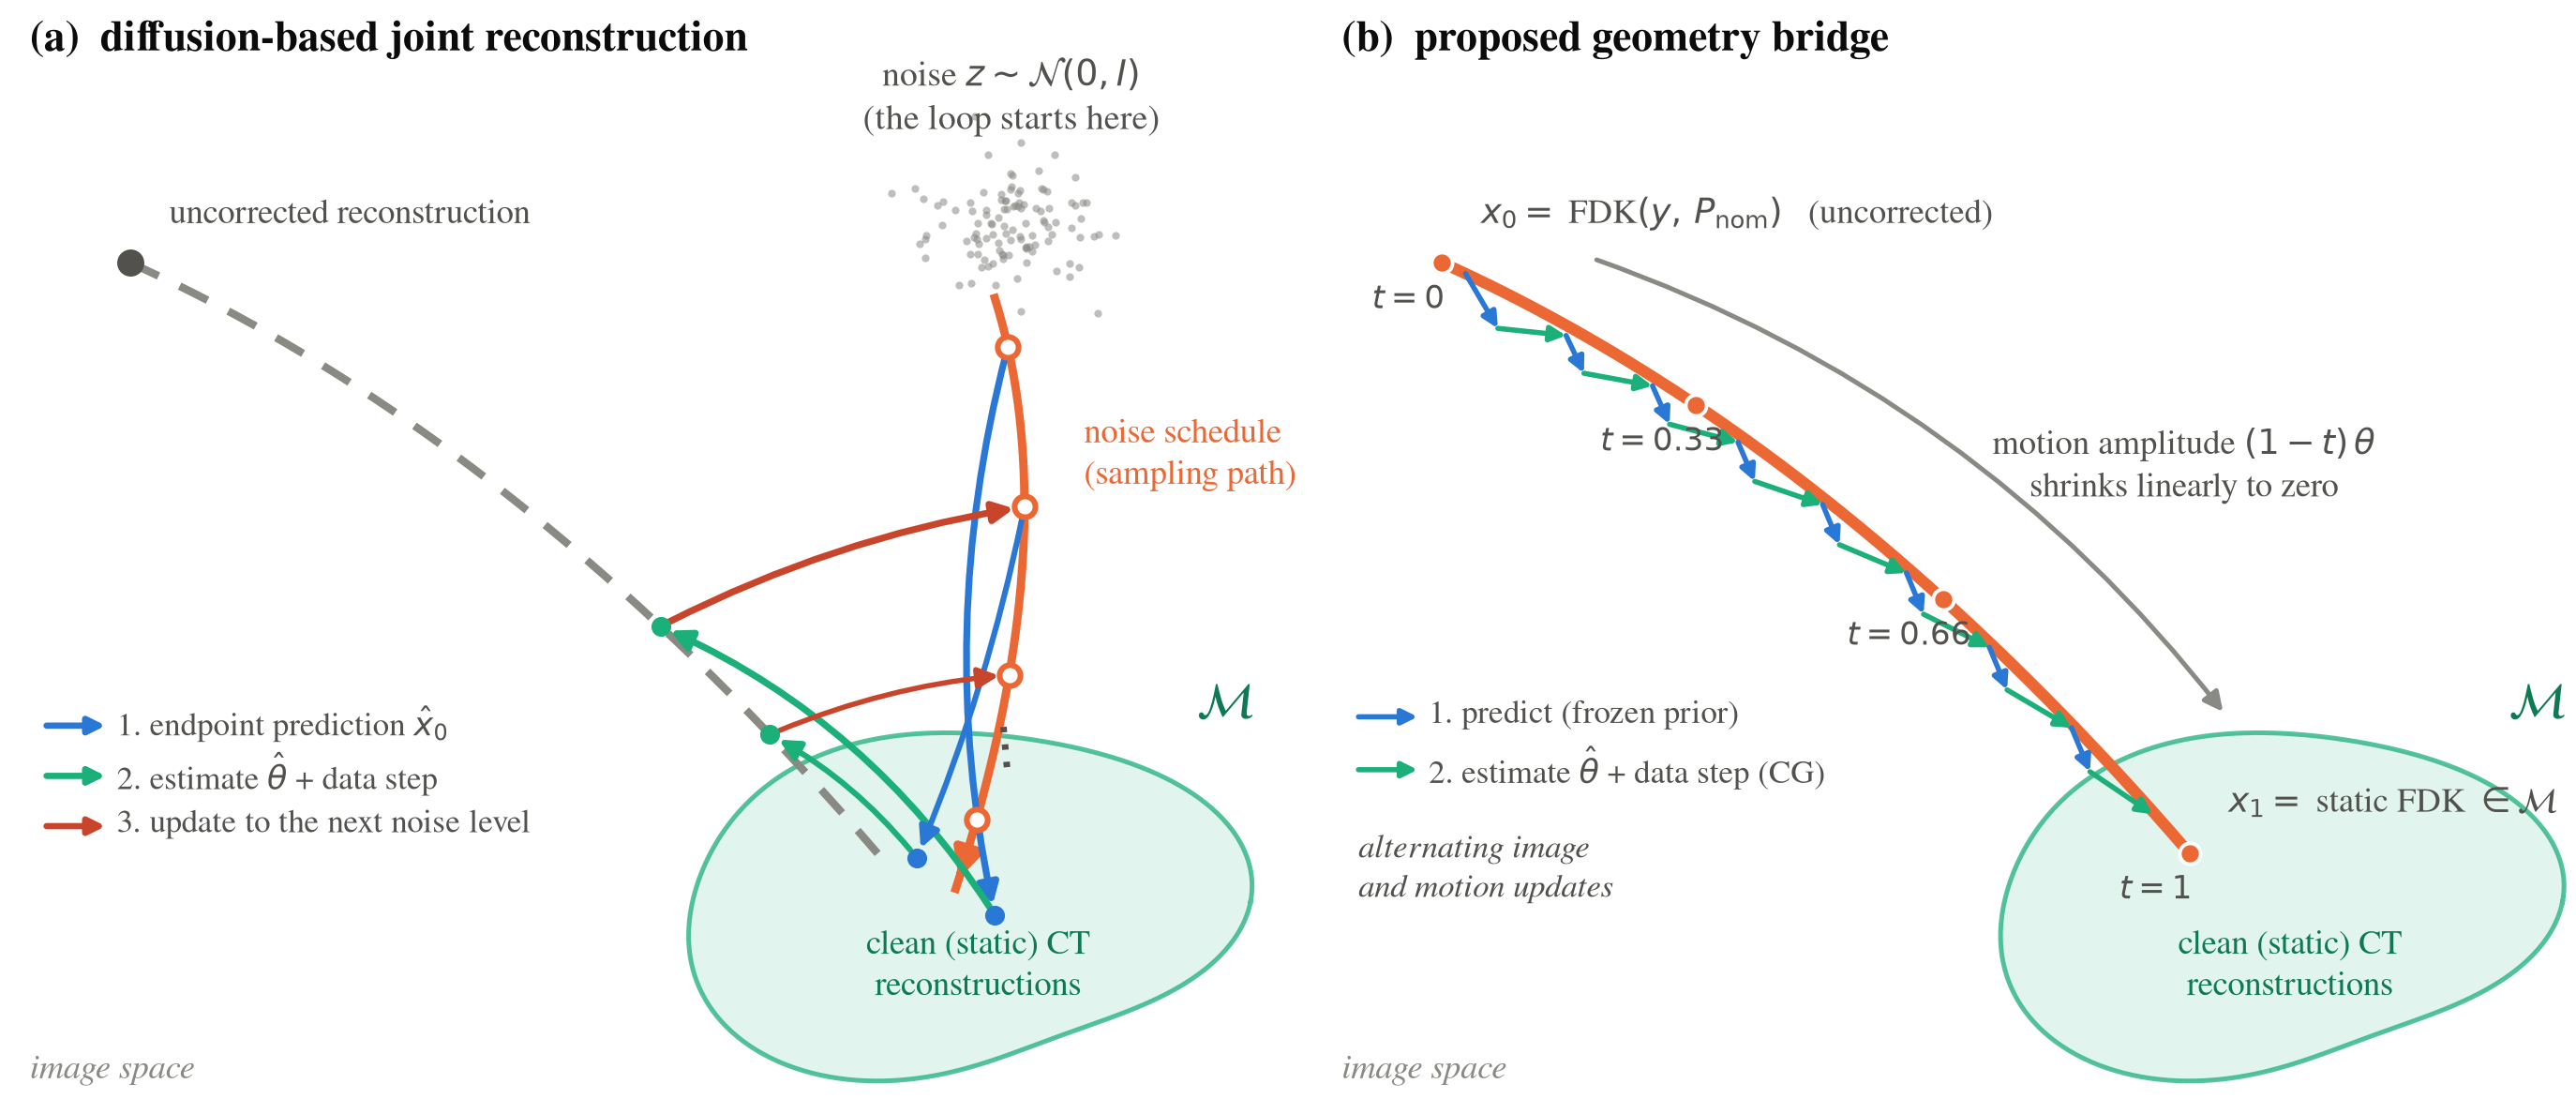
\includegraphics[width=0.95\textwidth]{fig0_manifold.png}
\caption{Figure 1: Schematic comparison of training paths and their use in joint reconstruction.
(a) A noise-to-clean diffusion prior predicts an image that is combined with motion and
data-consistency updates before advancing the sampling schedule. (b) The geometry
bridge consists of FDK reconstructions simulated with motion amplitude $(1-t)\theta$;
its tangent $dx_t/dt$ is the training target. The learned velocity guides image updates
interleaved with motion fitting and data consistency. The arrows illustrate the update
sequence, not measured inference trajectories or projection onto the training bridge.}


\end{figure}

The method has two main components: a 3D flow-matching prior on the geometry bridge,
with an analytic velocity target derived from the forward projector
(Sec.~II.B), and a predictor-corrector algorithm combining this prior with
hash-encoded motion estimation and conjugate-gradient data consistency
(Sec.~II.C). We evaluate image and motion recovery on 30 held-out patients
against learned autofocus and JRM-ADM, and compare the geometry bridge with a
pixel-linear path under the same training and inference settings
(Sec.~IV.B).\footnote{An earlier version of this work, without the
comparative evaluation, was submitted to SPIE Medical Imaging 2027.}

\section{II. Methods}


\subsection{A. Problem formulation}


Let $x$ denote an attenuation volume and $y$ the log-transformed projections acquired
over $V$ views on a nominal circular orbit $\Pnom$. The rigid pose at view $v$ is
$\theta_v\in\mathbb{R}^6$, comprising a translation and an axis-angle rotation.
Writing its transform as $T(\theta_v)$, the acquisition geometry is
$P(\theta)[v]=\Pnom[v]T(\theta_v)$ and the forward model is
$y=A_{P(\theta)}x$. We abbreviate this projector as $A_\theta$ and write
$\FDK(\theta)=\FDK(y,P(\theta))$ for analytic reconstruction at a given trajectory.

The image and motion updates are guided by the data-fidelity term
\begin{equation}
\mathcal{D}(x,\theta)=\tfrac12\|A_\theta x-y\|_2^2.

\end{equation}
We combine these updates with a learned flow velocity and total-variation (TV)
denoising. The learned prior enters through its image update, without specifying an
explicit regularization functional. The resulting iteration is described in
Sec.~II.C.

A common change of the object coordinate frame and acquisition geometry leaves the
projections unchanged. This SE(3) gauge ambiguity makes the absolute global pose
unobservable, so image and trajectory errors are evaluated after removing that offset
(Sec.~III.B).

\subsection{B. Flow-matching prior on the geometry bridge}


\begin{figure}[H]
\centering
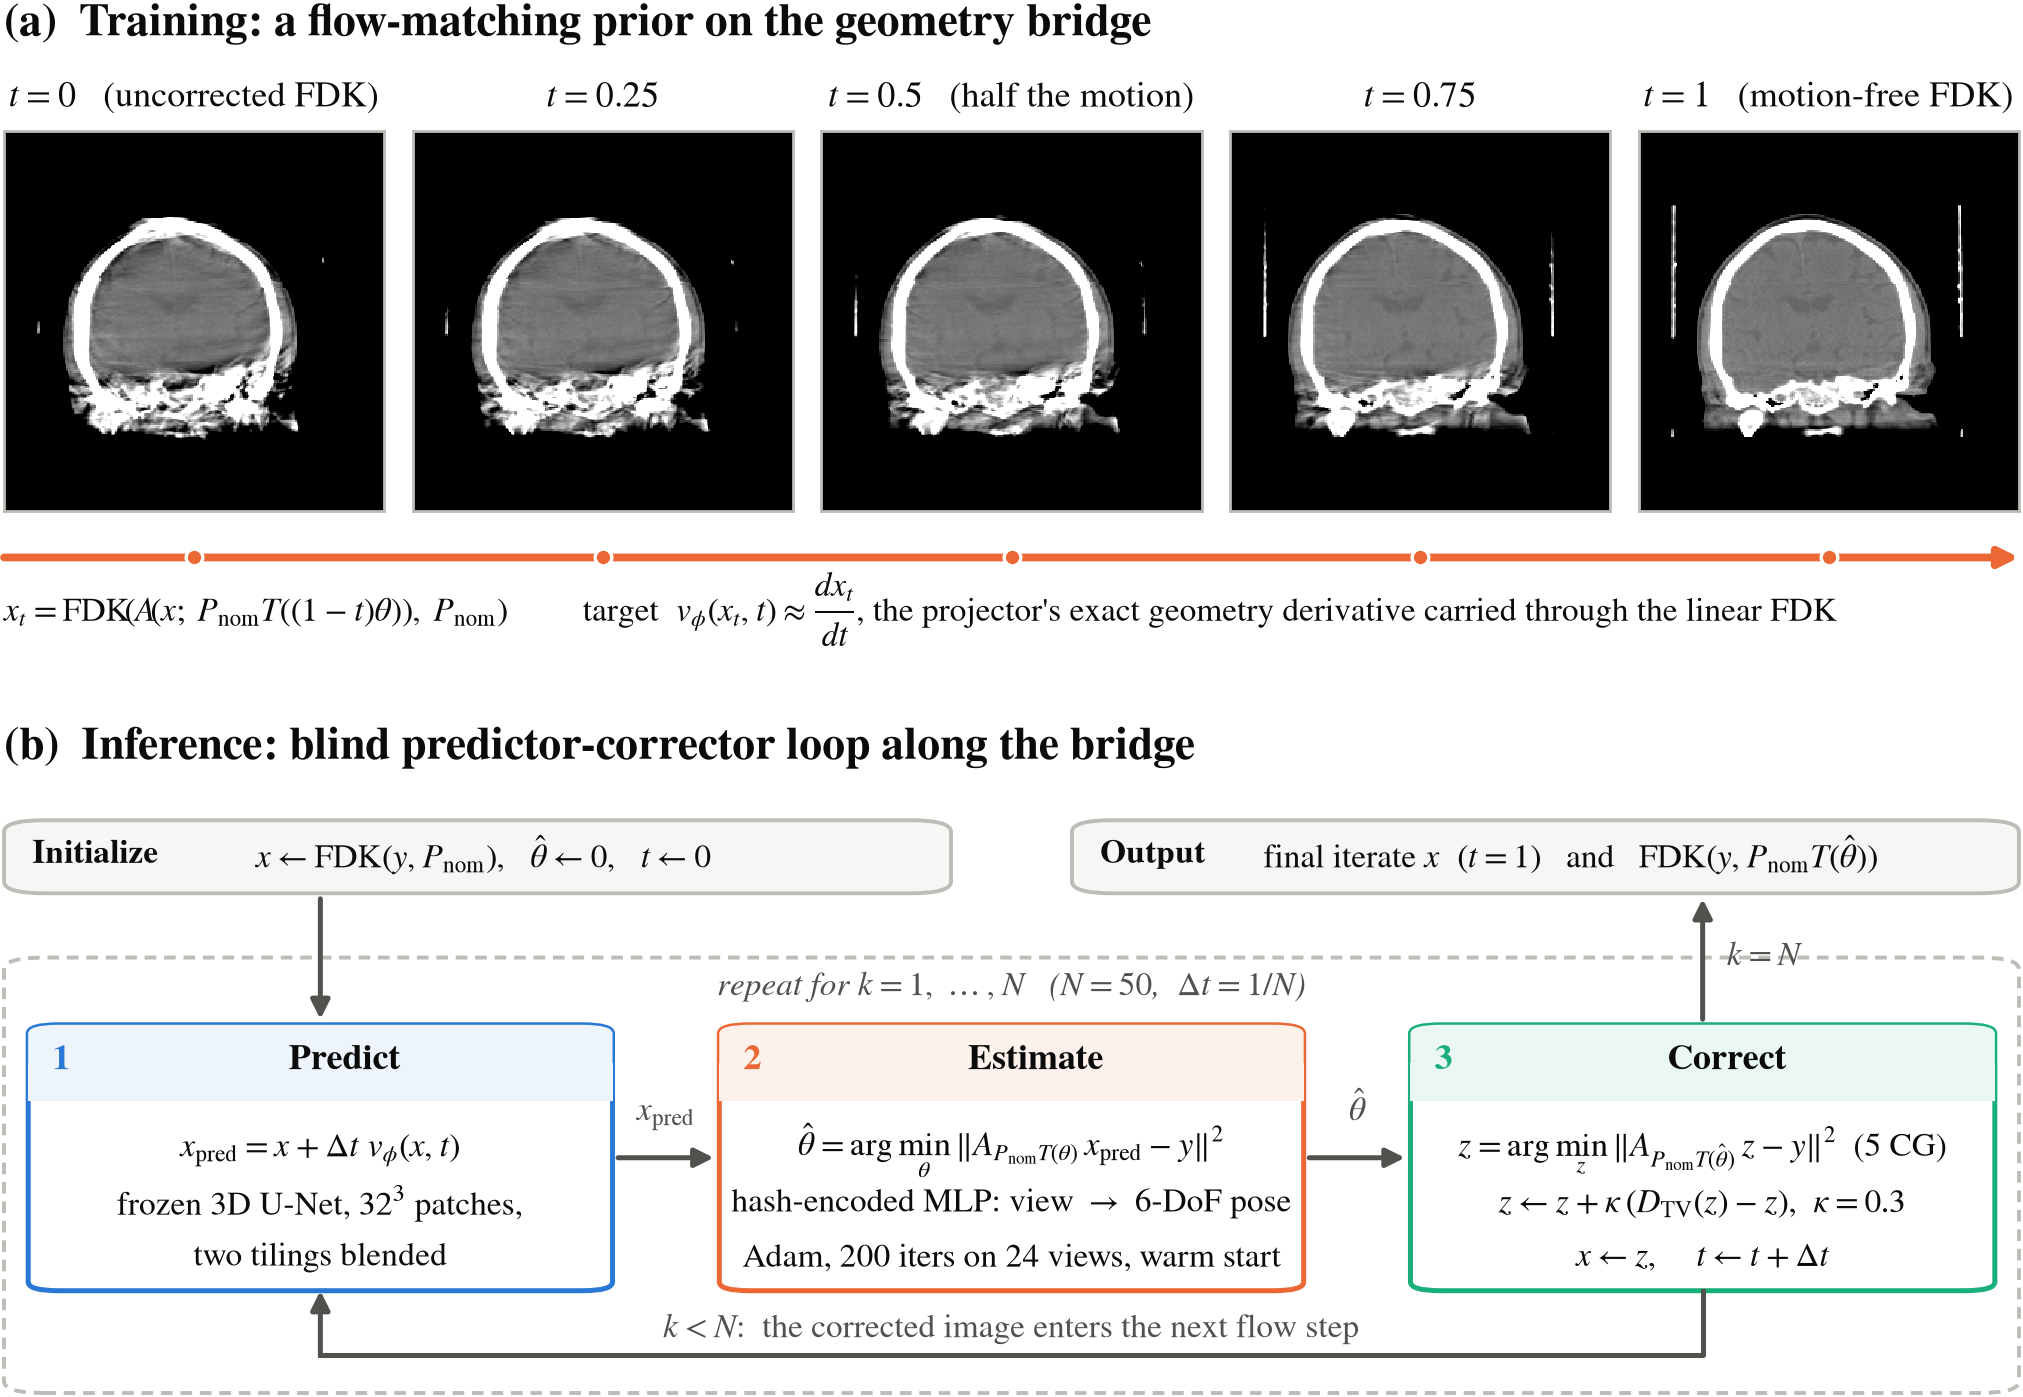
\includegraphics[width=0.80\textwidth]{fig1_method.png}
\caption{Figure 2: Training and inference. (a) FDK reconstructions of one volume re-simulated
with motion amplitude $(1-t)\theta$. The training target is the path tangent, obtained
by applying the fixed-geometry FDK operator to the projection derivative.
(b) At inference, the frozen prior predicts an image, the motion estimator fits the
measured projections to that prediction, and data consistency updates the image at
the estimated geometry.}


\end{figure}

Flow matching learns a velocity field $v_\phi(x,t)$ by regression to the tangent of a
prescribed path. For a training volume $x$ and simulated motion $\theta$, we define
the geometry bridge by reducing the motion amplitude and reconstructing each simulated
scan at the nominal geometry:
\begin{equation}
P_t=\Pnom T((1-t)\theta),\qquad
y_t=A_{P_t}x,\qquad x_t=\FDK(y_t,\Pnom).

\end{equation}
Scaling the translation and axis-angle rotation by $(1-t)$ reduces both to zero as
$t$ increases from 0 to 1. The initial state is the uncorrected reconstruction,
$x_0=\FDK(y,\Pnom)$, for the simulated scan $y=A_{P(\theta)}x$. The endpoint
$x_1=\FDK(A_{\Pnom}x,\Pnom)$ is its motion-free FDK counterpart. Intermediate
states are FDK reconstructions simulated at decreasing motion amplitudes
(Fig.~2(a)).

Since FDK is linear in its projection input and its reconstruction geometry is fixed,
the path tangent is
\begin{equation}
\dot x_t=\FDK(\dot y_t,\Pnom),\qquad
\dot y_t=D_P(A_Px)\big|_{P=P_t}[\dot P_t],\qquad
\dot P_t=\Pnom\frac{d}{dt}T((1-t)\theta).

\end{equation}
Here $D_P(A_Px)[\dot P_t]$ is the directional geometry derivative of the forward
projector. The rigid-transform derivative is analytic under the translation and
axis-angle parameterization, and the projector derivative is evaluated for the same
discrete operator used to generate the bridge. We train with the squared loss
$\|v_\phi(x_t,t)-\dot x_t\|_2^2$, sampling $t\sim\mathcal{U}[0,1]$.

The velocity field is represented by a 3D U-Net operating on $32^3$ patches.
Following[12], each patch receives four additional channels: the whole
current volume downsampled to $32^3$, and three maps of the patch voxels' absolute
$z$, $y$ and $x$ coordinates. These channels supply global anatomy and spatial context
while retaining the memory cost of patch-wise inference.

\subsection{C. Predictor-corrector inference loop}


Inference starts from the uncorrected reconstruction and zero motion. Each of $N=50$
iterations applies a prior prediction, refits the motion to that prediction, and updates
the image using the measured projections (Algorithm~1). The flow time
sets the input to the prior; the motion and data updates use the fixed measurement $y$.

\textbf{Algorithm 1: Blind rigid-motion correction with the geometry-bridge prior}

\begin{tabular}{l}
\hline
\textbf{Input:} projections $y$, nominal geometry $\Pnom$, frozen prior $v_\phi$, number of steps $N$ \\
1: $x\gets\FDK(y,\Pnom)$,  $\thetahat\gets0$,  $\Delta t\gets1/N$ \\
2: \textbf{for} $k=0,\dots,N-1$ \textbf{do} \\
3:  $t\gets k/N$,  $x_{\mathrm{pred}}\gets x+\Delta t\,v_\phi(x,t)$ \\
4:  $\thetahat\gets\mathrm{FitMotion}(x_{\mathrm{pred}},y;\thetahat)$   \textit{(warm-started Adam)} \\
5:  $z\gets\mathrm{CG}_5(A_{\thetahat},y;z_0=x_{\mathrm{pred}})$   \textit{(five data-update iterations)} \\
6:  $x\gets z+\kappa\,(D_{\mathrm{TV}}(z)-z)$   \textit{(relaxed TV update)} \\
7: \textbf{end for} \\
8: \textbf{return} final iterate $x_{\mathrm{final}}=x$ and $\FDK(\thetahat)$ \\
\hline
\end{tabular}


\textbf{Predict.} The frozen prior takes one Euler step,
$x_{\mathrm{pred}}=x+\Delta t\,v_\phi(x,t)$. Patch predictions are blended over two
tilings of the volume.

\textbf{Estimate.} The motion estimator fits the predicted image to the projections
by reducing $\|A_\theta x_{\mathrm{pred}}-y\|_2^2$. A multiresolution hash
encoding[13] maps the normalized view index to features, and an MLP
outputs the 6-DoF pose. We optimize the encoder and MLP with Adam, using the
projector's geometry gradient and retaining the optimizer state between flow steps.
No explicit trajectory smoothness penalty is used. Fitting the motion after the prior
update allows the estimator to use the current image correction.

\textbf{Correct.} At the updated trajectory $\thetahat$, five conjugate-gradient
(CG) iterations reduce the projection residual, initialized at $x_{\mathrm{pred}}$.
The resulting image $z$ receives a relaxed TV update,
$x=z+\kappa(D_{\mathrm{TV}}(z)-z)$, where $D_{\mathrm{TV}}$ denotes TV denoising.
This image becomes the input to the next prior prediction. The finite CG and motion
updates are not exact minimizations, and the corrected iterates need not lie on the
training bridge.

The algorithm returns the final iterate $x_{\mathrm{final}}$ and
$\FDK(\thetahat)$. The former is the reconstructed image after joint refinement;
the latter evaluates the estimated poses through analytic reconstruction. Although
FDK applies no learned image update, its poses were estimated with the aid of the prior.

\subsection{D. Implementation details}


The U-Net has base width 32, channel multipliers $(1,2,4)$, two residual blocks per
level, and a time embedding. It has 9.9M parameters and five input channels. We trained
it for 500k iterations using AdamW, a cosine learning-rate schedule from $10^{-4}$ to
$10^{-6}$, EMA 0.999, fp16, and 64 patches per batch.

Projection and backprojection use LEAP[14]. We implement the geometry
derivative of its forward operator for both the bridge target and motion estimation.
At each inference step, the motion estimator runs 200 Adam iterations with 24 randomly
sampled views per iteration. It uses half volume resolution until $t=0.5$ and full
resolution thereafter. The data update uses five CG iterations, followed by five TV
iterations with step size 0.015 and relaxation weight $\kappa=0.3$.
Source code is available at \url{https://github.com/dbstjstod1/Flow_matching_motion_3D}.

\section{III. Experiments}


\subsection{A. Data and simulation setup}


We use the CQ500 head CT collection[15], selecting one thin-slice series per
patient and removing slice-count outliers following[2]. Of the 343
retained patients, 150 are assigned to training, 50 to validation and 143 to the test
split. Reconstructions use a $256^3$ grid with 1\,mm voxels.

Projections are simulated as noiseless line integrals on a finer $612^3$ grid with
0.42\,mm voxels to reduce dependence on the reconstruction discretization. The
head-CBCT geometry follows[2]: source-isocenter distance 785\,mm,
source-detector distance 1200\,mm, a $700\times500$ detector with 0.64\,mm pixel
pitch, and 360 views over a full rotation. Photon noise, scatter and beam hardening
are not modeled.

For each motion component, a zero-centered Akima spline[16] is drawn through
10 random nodes. Training samples per-component amplitudes up to
15\,mm\,/\,20°; evaluation uses one fixed
10\,mm\,/\,10° pattern per patient. All amplitudes are peak-to-peak.
The evaluation uses the same $[-5,5]$\,mm and degree control-point range as
[7], with a different spline interpolant, and twice the motion amplitude
reported in the evaluation of[2].

\subsection{B. Evaluation protocol}


We evaluate 30 patients from the held-out test split, following the cohort size
of[2]. Each method receives the same patient, motion realization and
sinogram, giving paired comparisons. Before computing PSNR and SSIM, reconstructed
volumes are rigidly aligned to the ground truth to account for the global pose
ambiguity. Both metrics are evaluated within the measured field of view for all methods.

Motion accuracy is assessed by reprojection error (RPE)[2], the mean
detector displacement induced by pose error over a set of points in the head.
Trajectories are placed in a zero-mean gauge before comparison. We also report the
mean absolute error of each motion component over views and patients, in millimeters
for translation and degrees for rotation. These component-wise errors complement RPE,
which combines the six pose components into a detector-plane displacement.
Analytic reconstructions at the estimated poses provide an additional image-domain
assessment. Reported $p$-values use paired two-sided Wilcoxon signed-rank tests.

\subsection{C. Comparison methods}


\paragraph{Learned autofocus[2].}
Thies et al. estimate motion by maximizing a learned image-quality metric. A network
predicts a voxel-wise VIF map from the reconstruction, and gradient descent adjusts
the spline control points through a differentiable backprojector. The method returns
an analytic reconstruction at the estimated poses and uses no projection-domain
data-fidelity term. We use the authors' released implementation and reconstruction
operator, with the quality network retrained on our 150 training patients.

\paragraph{JRM-ADM[7].}
JRM-ADM combines a Haar-wavelet diffusion prior (W3DM[17]) with joint image
and motion updates. At each sampling step, the prior predicts a clean volume;
weighted-least-squares projection fitting then updates the image and the 6-DoF motion,
parameterized by cubic B-spline control points. We use the authors' released sampler
and optimizers, with the prior retrained on our 150 training patients under their
noise schedule. For our full-view protocol, the reconstruction grid is extended to
$224^3$ and the prior weight is rescaled to preserve the data-to-prior balance.
The reconstructed volume is placed in the evaluation frame and the poses are converted
to our geometry convention for scoring. This evaluates the method under our 360-view
protocol, rather than reproducing its published sparse-view experiment.

\paragraph{Bridge ablation (pixel-linear bridge).}
We train a second prior on the pixel-linear path $x_t=(1-t)x_0+t x_1$, with target
velocity $x_1-x_0$. The endpoints, U-Net, conditioning channels, time sampling, 500k
training iterations and inference loop are unchanged. This comparison tests the
geometry-based path and its tangent against linear interpolation under a fixed
training and inference configuration.

\section{IV. Results}


\subsection{A. Performance of the proposed method}


\begin{figure}[H]
\centering
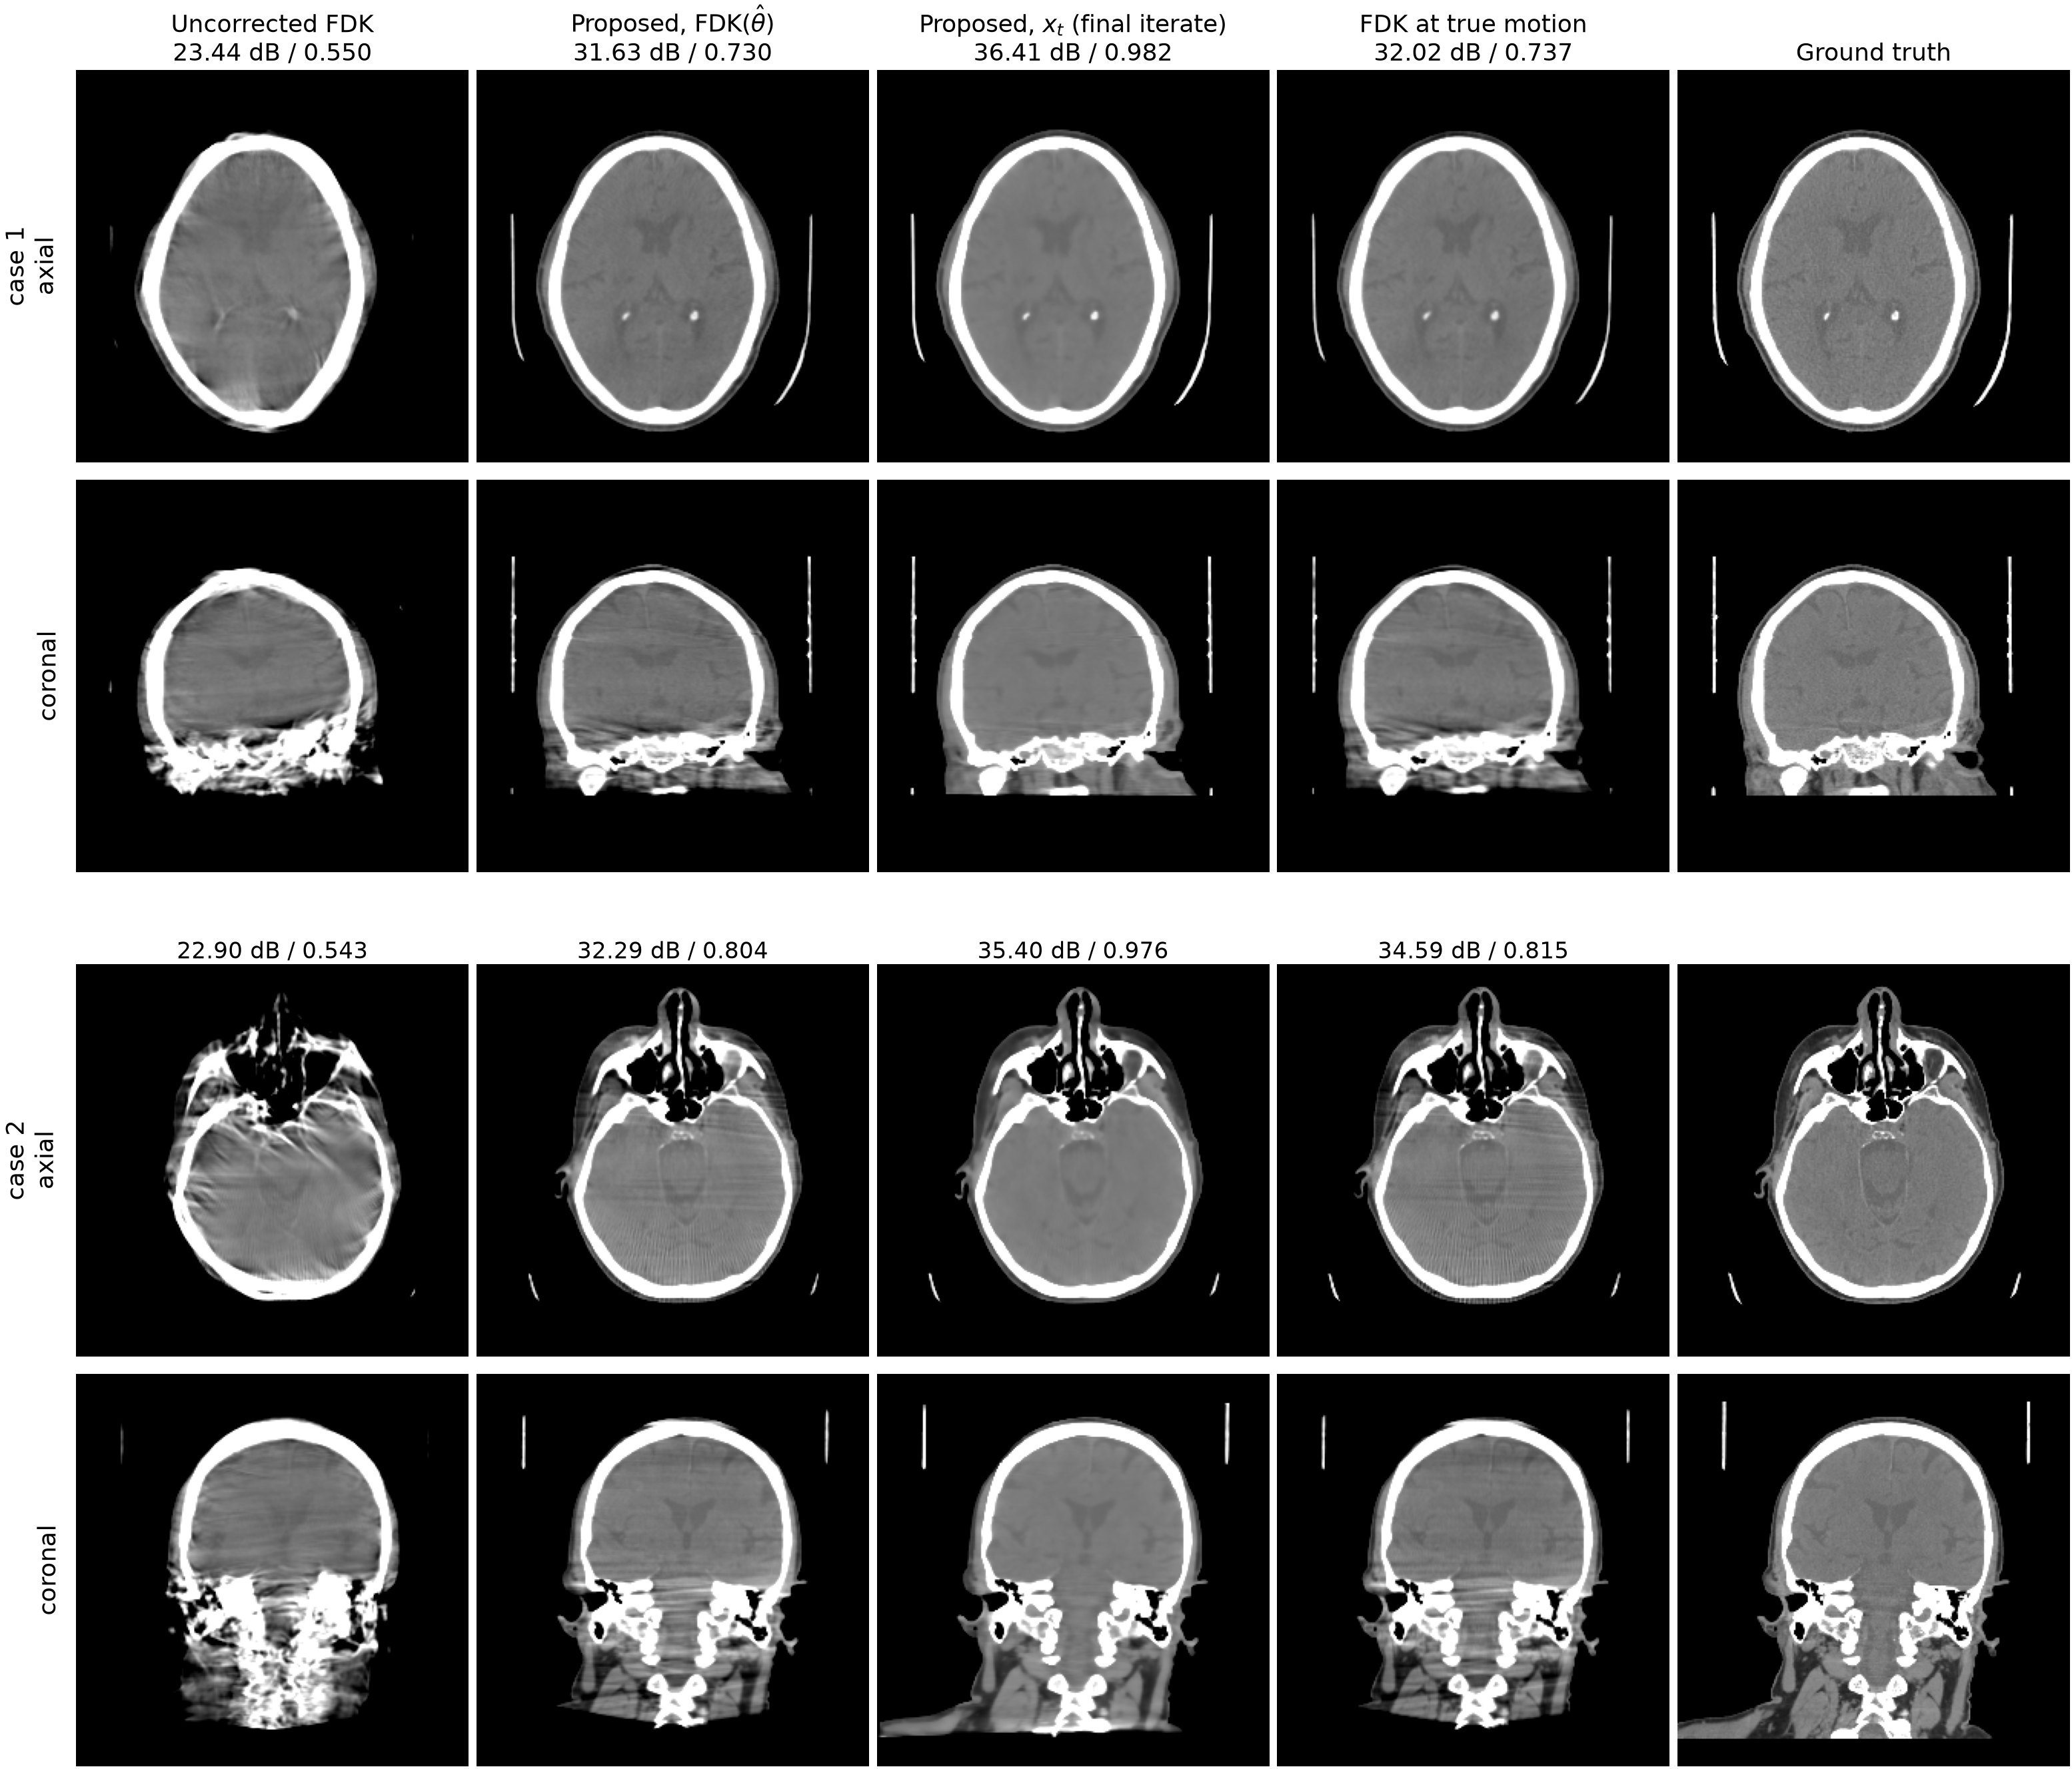
\includegraphics[width=0.92\textwidth]{fig_ours_qual.png}
\caption{Figure 3: Two representative test patients at 10\,mm\,/\,10° motion, brain window
(level 40\,/\,width 420\,HU); volumes are rigidly aligned to the ground truth before
display, and labels give PSNR\,/\,SSIM against the ground-truth volume. The fourth column
is the FDK of the same scan at the true motion.}

\end{figure}

\begin{table}[H]
\centering
\caption{Table 1: Performance of the proposed method on 30 held-out CQ500 patients with Akima
motion at 10\,mm\,/\,10° peak-to-peak. PSNR and SSIM are computed against the
ground-truth volume after rigid alignment, within the measured field of view; RPE is the
reprojection error of[2] with the mean pose offset removed (mean $\pm$
standard deviation).}

\begin{tabular}{lccc}
\toprule
Output & PSNR (dB) & SSIM & RPE (mm) \\
\midrule
Uncorrected FDK & 23.29 $\pm$ 0.93 & 0.546 $\pm$ 0.035 & 6.12 $\pm$ 0.66 \\
FDK($\thetahat$) & 31.80 $\pm$ 0.76 & 0.753 $\pm$ 0.032 & 0.28 $\pm$ 0.09 \\
\textbf{$x_{\mathrm{final}}$ (final iterate)} & \textbf{36.66 $\pm$ 1.58} & \textbf{0.978 $\pm$ 0.008} & \textbf{0.28 $\pm$ 0.09} \\
\bottomrule
\end{tabular}
\end{table}

\begin{figure}[H]
\centering
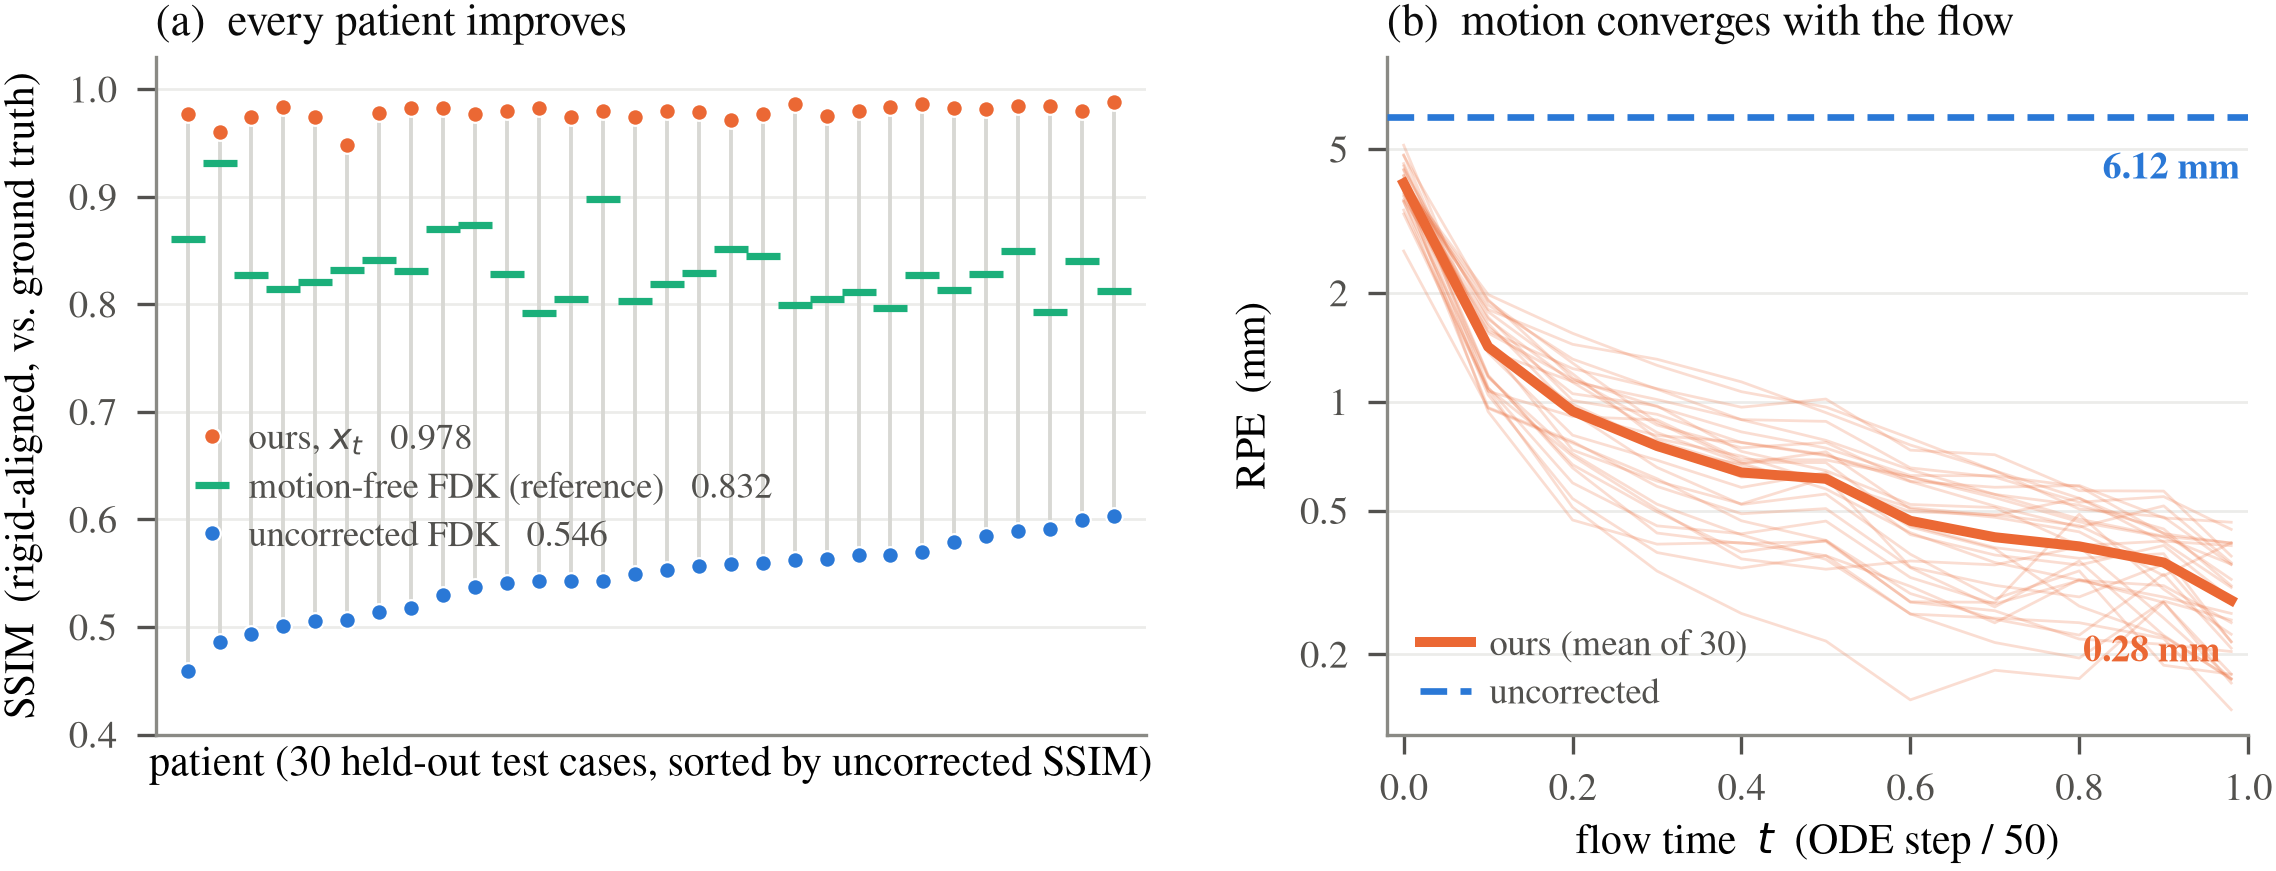
\includegraphics[width=0.78\textwidth]{fig3_quant.png}
\caption{Figure 4: Cohort results over 30 held-out patients. (a) Per-patient SSIM; grey stems join
each patient's uncorrected and corrected score. (b) Reprojection error against flow time
(thin: individual patients).}

\end{figure}

The final iterate achieved 36.66\,dB PSNR and 0.978 SSIM, compared with
23.29\,dB and 0.546 for the uncorrected FDK (Table~1). Image quality
improved in all 30 patients (Fig.~4(a)), and mean RPE decreased from
6.12 to 0.28\,mm over the iteration (Fig.~4(b)). Inference took
9.3 minutes per patient on one RTX A6000 GPU (Sec.~IV.C).

The analytic reconstruction at the estimated poses reached 31.80\,dB and 0.753 SSIM.
In the displayed cases, it resembles FDK at the true motion, with residual artifacts
in both analytic images (Fig.~3). The final iterate improves on
$\FDK(\thetahat)$ by 4.9\,dB and 0.225 SSIM. It also exceeds the motion-free
FDK reference, obtained from a separately simulated static acquisition at the nominal
geometry (33.11\,dB and 0.832 SSIM), by 3.5\,dB and 0.146 SSIM. This gain shows
the benefit of iterative reconstruction beyond analytic motion compensation.

\FloatBarrier
\subsection{B. Comparison with other methods}


\begin{figure}[H]
\centering
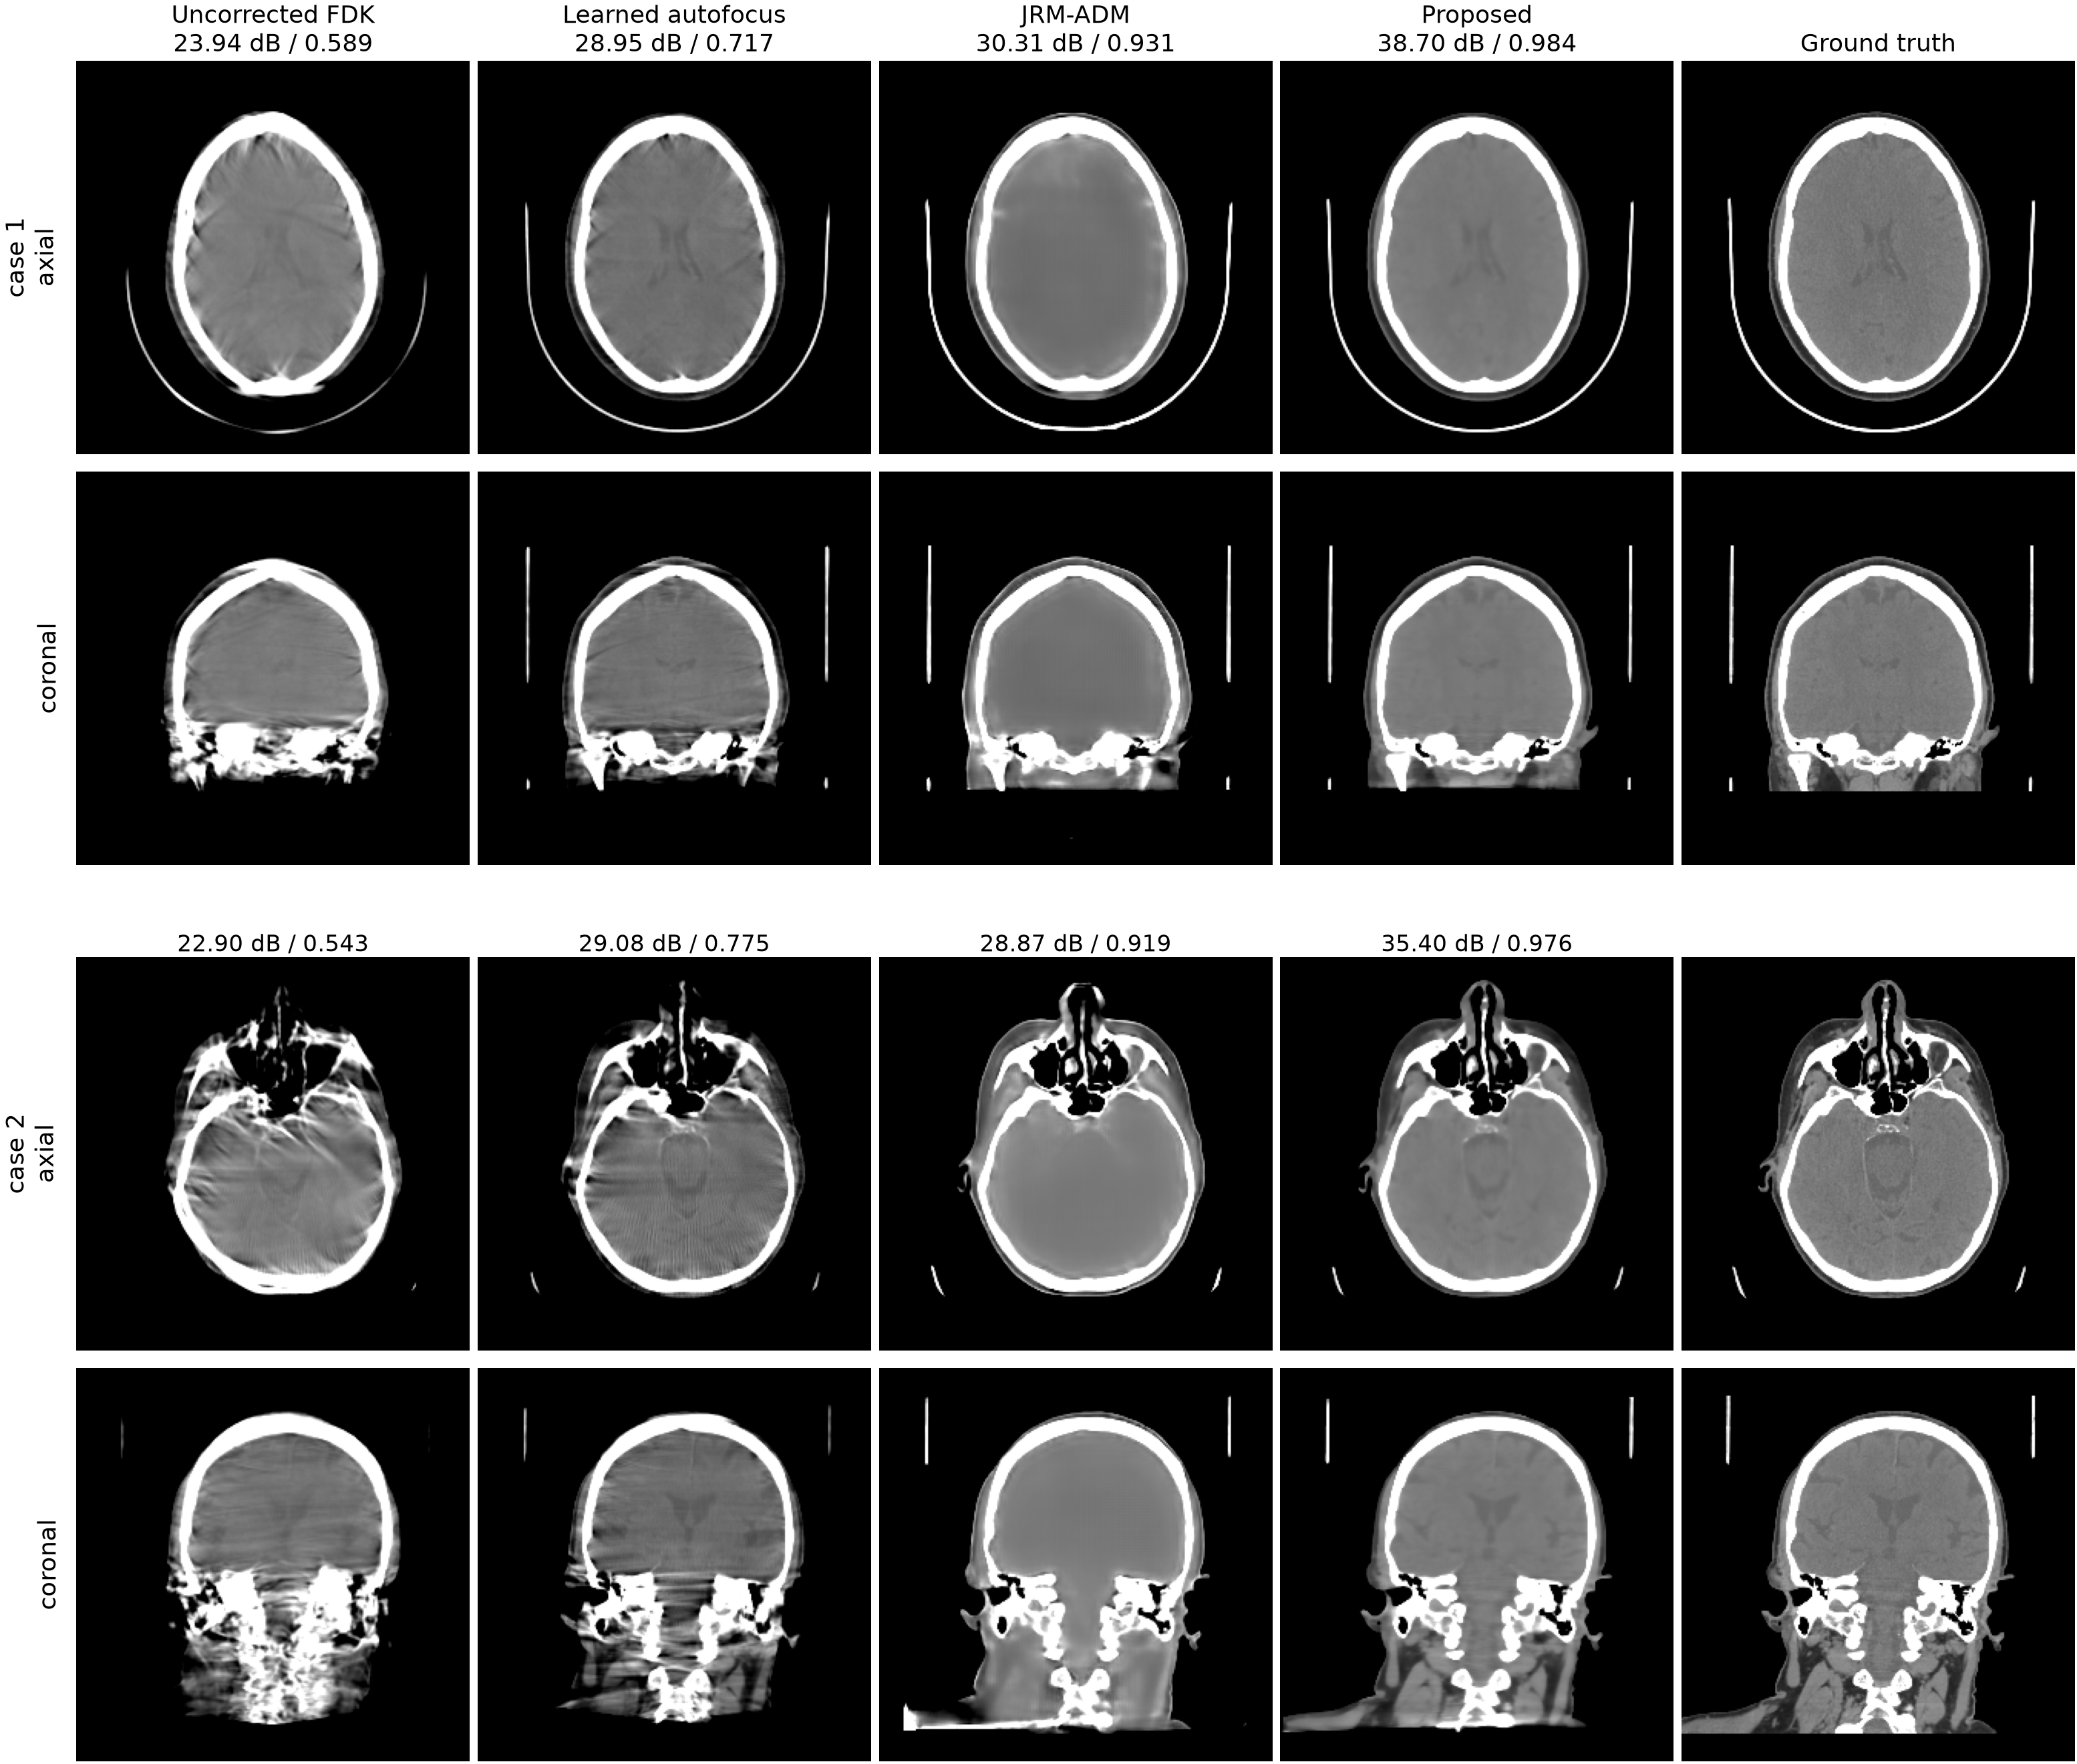
\includegraphics[width=0.80\textwidth]{fig4_bench.png}
\caption{Figure 5: Qualitative comparison on two representative test patients, axial and coronal
slices in the brain window; the axial slice of the second case lies at the skull-base level.
All volumes are rigidly aligned to the ground truth before slicing, and labels give
PSNR\,/\,SSIM against the ground truth.}

\end{figure}

\begin{table}[H]
\centering
\caption{Table 2: Comparison with other methods on the same 30 patients, under the conventions
of Table~1. All learned components were retrained on the same 150 training
patients and evaluated on identical (patient, motion, sinogram) triples. The pixel-linear row is the bridge
ablation discussed at the end of this section.}

\begin{tabular}{lccc}
\toprule
Method & PSNR (dB) & SSIM & RPE (mm) \\
\midrule
Learned autofocus[2] & 29.22 $\pm$ 1.11 & 0.727 $\pm$ 0.032 & 2.26 $\pm$ 0.52 \\
JRM-ADM[7] & 29.64 $\pm$ 2.64 & 0.912 $\pm$ 0.038 & 0.84 $\pm$ 0.55 \\
Proposed, FDK($\thetahat$) & 31.80 $\pm$ 0.76 & 0.753 $\pm$ 0.032 & 0.28 $\pm$ 0.09 \\
Proposed, pixel-linear bridge (ablation) & 35.29 $\pm$ 2.28 & 0.966 $\pm$ 0.015 & 0.42 $\pm$ 0.17 \\
\textbf{Proposed, $x_{\mathrm{final}}$ (final iterate)} & \textbf{36.66 $\pm$ 1.58} & \textbf{0.978 $\pm$ 0.008} & \textbf{0.28 $\pm$ 0.09} \\
\bottomrule
\end{tabular}
\end{table}

The proposed method reduced RPE relative to learned autofocus in all 30 patients,
from a cohort mean of 2.26 to 0.28\,mm ($p=1.7\times10^{-6}$;
Table~2). Its analytic output also exceeded the autofocus reconstruction:
PSNR was higher by 2.6\,dB on average and in all 30 patients, while SSIM was higher
by 0.026 on average and in 23 patients ($p=1.5\times10^{-4}$ for SSIM).
The final iterate exceeded the autofocus output in both image metrics for all patients.
In Fig.~5, autofocus reduces the motion artifacts but leaves visible
streaks, particularly in the coronal slices.

\begin{figure}[H]
\centering
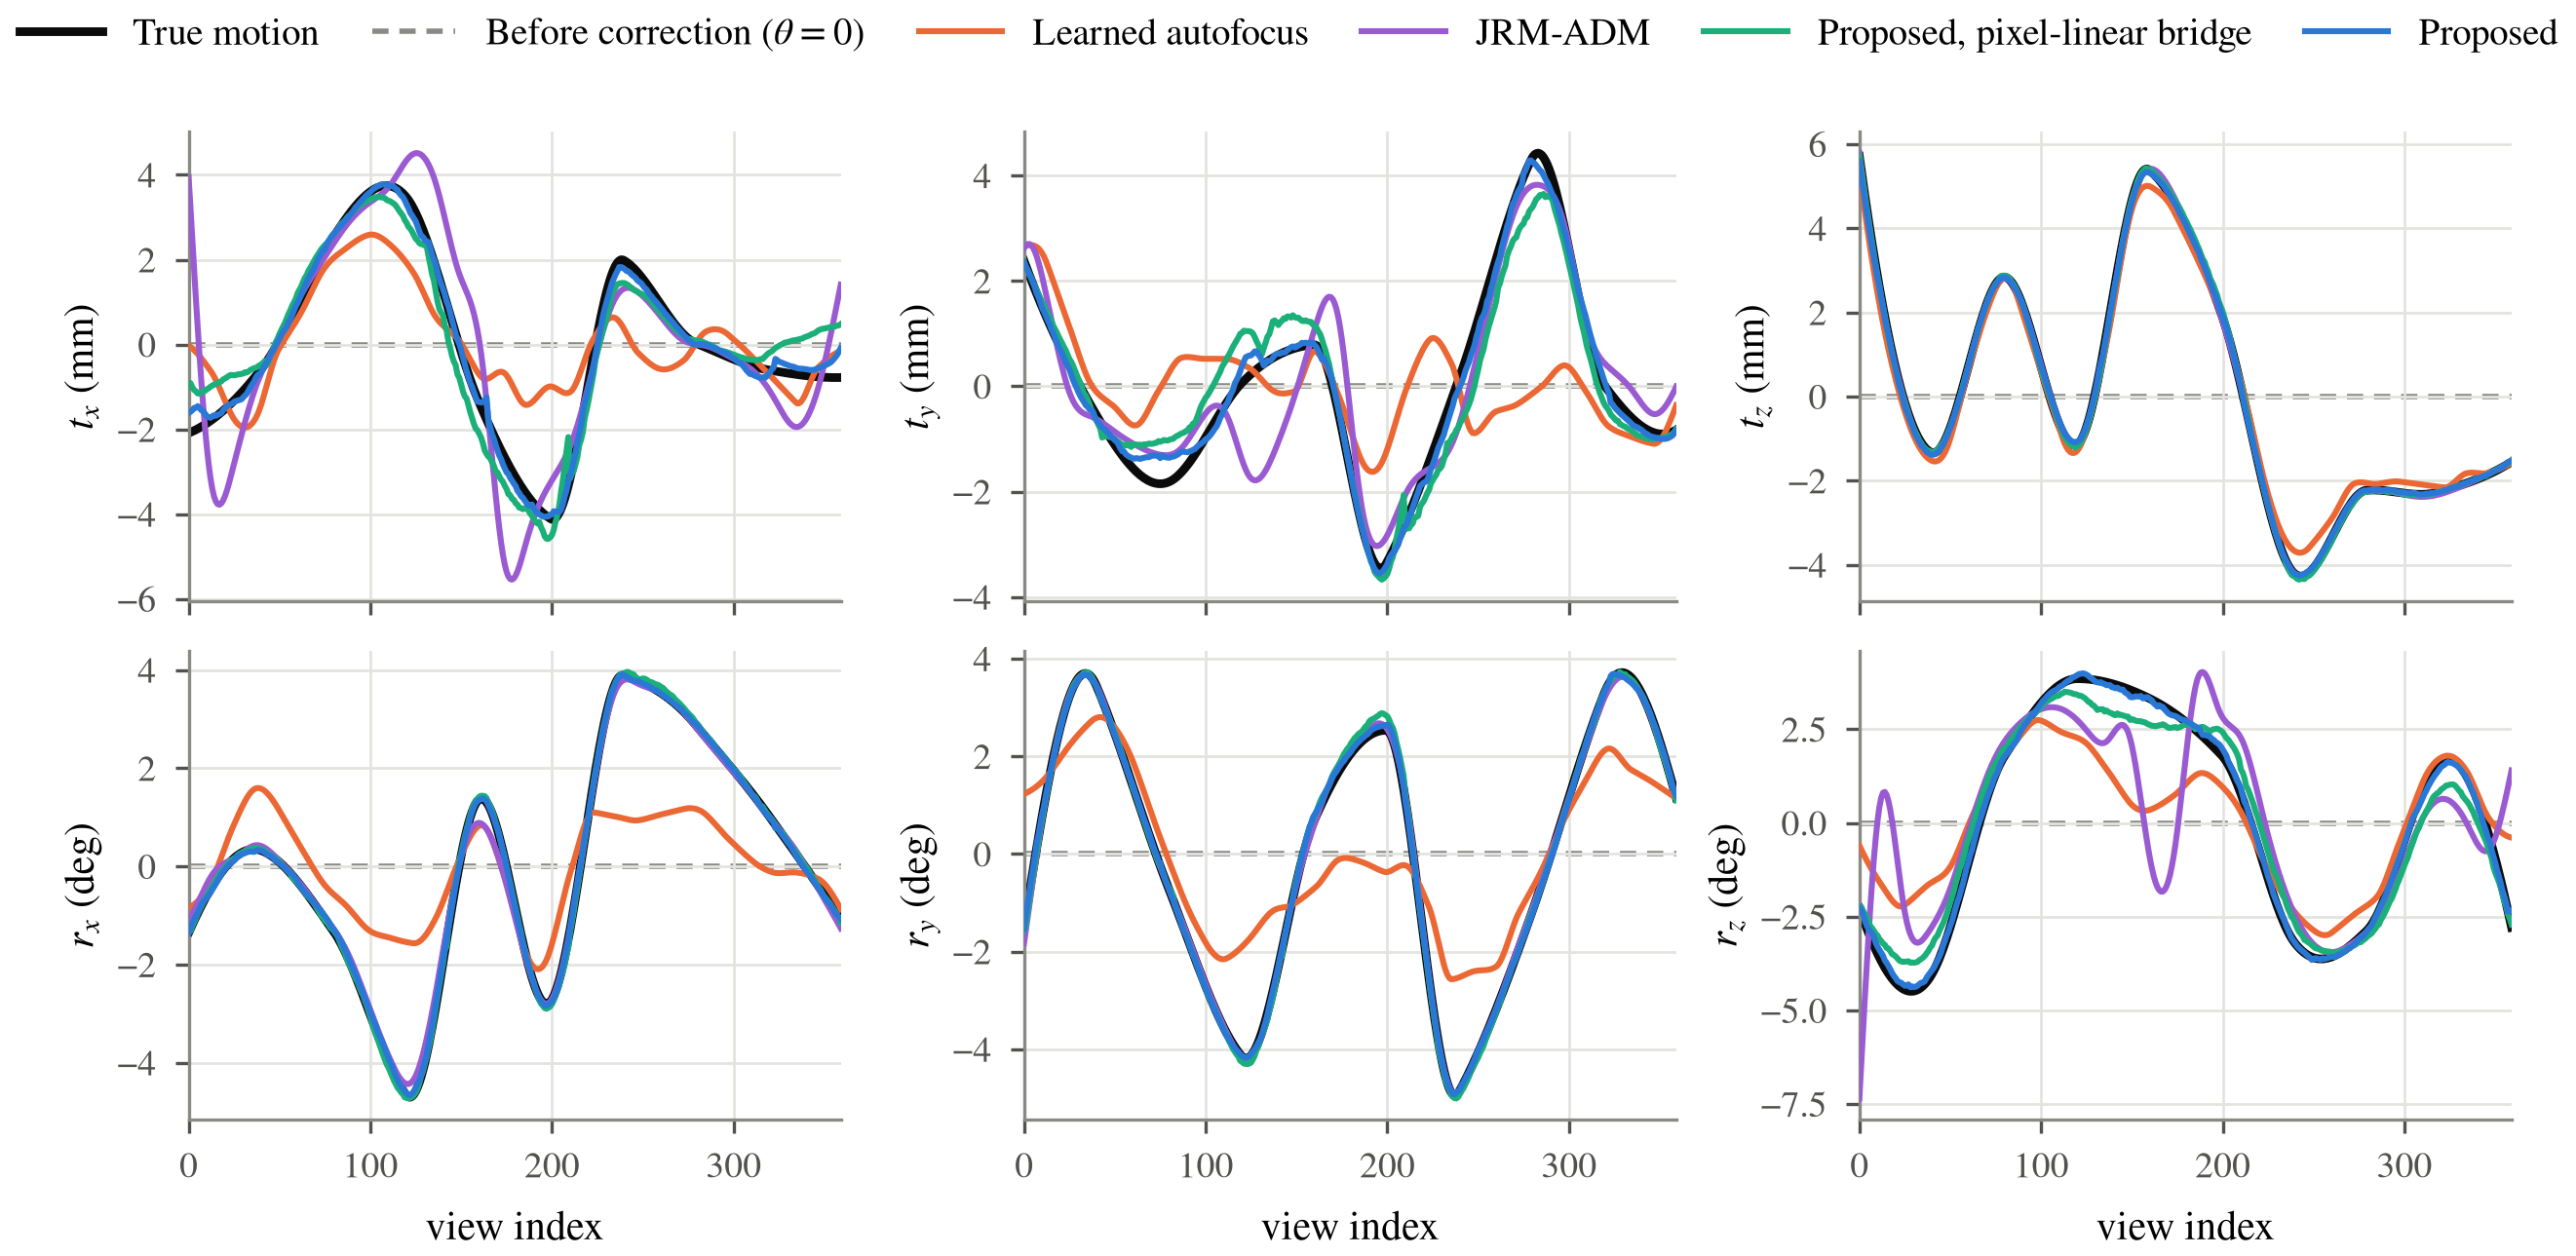
\includegraphics[width=\textwidth]{fig_motion.png}
\caption{Figure 6: Recovered motion of one test patient (the first case of Fig.~5).
Each panel shows one degree of freedom against the view index: the true trajectory, the
state before correction ($\theta=0$), and the trajectory recovered by each method, all on
the zero-mean gauge. Translations in mm, rotations in degrees.}

\end{figure}

\begin{table}[H]
\centering
\caption{Table 3: Per-DoF mean absolute error of the recovered motion over the 30 patients, on the
zero-mean gauge. Translations in mm, rotations in degrees. Bold values denote
column minima at the reported precision.}

\small
\begin{tabular}{lcccccc}
\toprule
Method & $t_x$ & $t_y$ & $t_z$ & $r_x$ & $r_y$ & $r_z$ \\
\midrule
Uncorrected & 1.93 & 2.08 & 1.95 & 2.01 & 1.90 & 2.17 \\
Learned autofocus[2] & 1.30 & 1.33 & 0.36 & 0.95 & 0.98 & 1.09 \\
JRM-ADM[7] & 2.17 & 1.97 & 0.06 & 0.09 & 0.07 & 0.68 \\
Proposed, pixel-linear bridge (ablation) & \textbf{0.71} & \textbf{0.69} & 0.04 & \textbf{0.04} & 0.05 & 0.40 \\
\textbf{Proposed} & 0.79 & 0.78 & \textbf{0.03} & \textbf{0.04} & \textbf{0.04} & \textbf{0.23} \\
\bottomrule
\end{tabular}
\end{table}

The component-wise errors reveal differences that are less apparent in RPE alone
(Table~3). The proposed method reduced translation MAE to at most
0.79\,mm and rotation MAE to at most 0.23°. Its largest residual errors were
in the in-plane translations and gantry-axis rotation. The pixel-linear prior had
slightly lower in-plane translation errors, while the geometry bridge had lower
gantry-axis rotation error (0.23° versus 0.40°).
Fig.~6 shows these trajectories for one patient.

JRM-ADM recovered axial translation and out-of-plane rotations with low error, but
its in-plane translation MAEs were 2.17 and 1.97\,mm despite an RPE of 0.84\,mm.
This discrepancy is consistent with drift along directions to which detector-plane
displacement is less sensitive. RPE and component-wise pose errors therefore provide
complementary assessments of motion recovery.

JRM-ADM's final reconstruction achieved 29.64\,dB and 0.912 SSIM, compared with
36.66\,dB and 0.978 for the proposed method. The PSNR gain was present in all
30 patients ($p=1.9\times10^{-9}$). FDK at the JRM-ADM poses reached
29.45\,dB and 0.715 SSIM; the proposed analytic output had higher PSNR in 28
patients, with a mean gain of 2.3\,dB ($p=1.6\times10^{-7}$).
The displayed JRM-ADM reconstructions suppress much of the motion artifact but show
more smoothing of soft-tissue contrast than the proposed output
(Fig.~5).

With the pixel-linear bridge, final PSNR and SSIM decreased to 35.29\,dB and 0.966,
and RPE increased to 0.42\,mm (Table~2). The geometry bridge improved
PSNR by approximately 1.4\,dB and SSIM by 0.012 under the same training and inference
settings. This ablation supports the choice of a path defined by simulated motion
reduction, while the component-wise results show that the improvement is not uniform
across all pose parameters.

\FloatBarrier
\subsection{C. Computational cost}


\begin{table}[H]
\centering
\caption{Table 4: Computational cost. Proposed and JRM-ADM runtimes were measured on an RTX A6000
under the 360-view protocol; the autofocus runtime is reported by its authors.
Network evaluations count complete prior or quality evaluations, including patch-wise
processing for the proposed method. Operator counts are approximate full-view
equivalents: an update using 24 views contributes $24/360$. Different resolutions and
operators give these updates different computational costs.}


\small
\begin{tabular}{lccc}
\toprule
Method & Network evaluations & Full-view equivalents & Time \\
\midrule
Learned autofocus[2] & 100 & $\sim$100 & $<2$\,min (reported) \\
JRM-ADM[7] & 100 & $\sim$1{,}600 & 4.6\,h \\
Proposed & 50 & $\sim$900 & 9.3\,min \\
\bottomrule
\end{tabular}
\end{table}

The proposed method took 9.3 minutes per patient, with approximately 80\% of the
runtime spent in motion estimation. Its 10,000 Adam iterations use 24 views each,
amounting to roughly 670 full-view equivalents; the 250 CG iterations add another
250. Half-resolution motion fitting during the first half of inference further reduces
the cost. The learned autofocus method requires fewer updates and has a published
runtime below two minutes (Table~4).

JRM-ADM took 4.6 hours per patient in this implementation. Its 100 sampling steps
use 10--15 image updates and 5--10 motion updates per step, each over all 360 views,
for approximately 1,600 full-view equivalents. This count is less than twice that of
the proposed method, so update counts alone do not explain the runtime difference.
The comparison also includes different projector implementations, resolutions and
solver costs. In particular, the 360-view protocol increases the work per data update
relative to JRM-ADM's sparse-view setting; the measured runtime difference should be
interpreted within this protocol.

\FloatBarrier
\section{V. Discussion}


The geometry bridge gives the prior a training target tied to a specified reduction in
motion. Its advantage over the pixel-linear path, with architecture and inference held
fixed, supports using the simulated acquisition model to define the training path.
The learned velocity can then guide image updates before motion fitting. The inference
iterates also include data-consistency and TV updates, however, so they are not required
to follow the prescribed training path exactly.

The two outputs distinguish image reconstruction from evaluation of the recovered poses.
FDK at the estimated poses permits comparison through an analytic reconstruction,
while the final iterate includes the effects of joint image refinement. The gain over
motion-free FDK shows that reconstruction quality can improve beyond that analytic
reference. It does not determine how much residual motion still limits the iterative
result. Likewise, the comparison with JRM-ADM establishes a difference between complete
methods under a common evaluation protocol, without attributing that difference to a
single component.

The evidence is limited to noiseless simulated projections, one rigid-motion realization
per test patient, and the specified acquisition geometry. Photon noise, scatter, beam
hardening and genuine patient motion require evaluation on measured data. The rigid
model is appropriate for the skull but does not describe independent mandibular or neck
motion. The baseline comparisons also differ from their published evaluation settings:
autofocus is tested at a larger motion amplitude, and JRM-ADM is applied to full-view
data. Finally, the 9.3-minute runtime remains longer than the reported autofocus runtime.
Reducing the cost of motion fitting is the main opportunity for acceleration in the
current implementation.

\section{VI. Conclusion}


We presented a 3D flow-matching prior trained on FDK reconstructions with progressively
reduced motion and integrated it into joint image and pose estimation. On simulated
scans from 30 held-out patients, the method achieved 36.66\,dB PSNR, 0.978 SSIM and
0.28\,mm reprojection error, improving image quality and motion accuracy relative to
learned autofocus and JRM-ADM under the tested protocol. The pixel-linear ablation
supports the geometry bridge as a training path for this reconstruction problem.

\section*{References}

[1] A.~Sisniega, J.~W. Stayman, J.~Yorkston, J.~H. Siewerdsen, and W.~Zbijewski, ``Motion compensation in extremity cone-beam CT using a penalized image sharpness criterion,'' \emph{Phys. Med. Biol.} \textbf{62}(9), 3712--3734 (2017).


[2] M.~Thies et al., ``A gradient-based approach to fast and accurate head motion compensation in cone-beam CT,'' \emph{IEEE Trans. Med. Imaging} \textbf{44}(2), 1098--1109 (2025).


[3] H.~Huang, J.~H. Siewerdsen, W.~Zbijewski, C.~R. Weiss, T.~Ehtiati, and A.~Sisniega, ``Reference-free learning-based similarity metric for motion compensation in cone-beam CT,'' \emph{Phys. Med. Biol.} \textbf{67}(12), 125020 (2022).


[4] Y.~Ko, S.~Moon, J.~Baek, and H.~Shim, ``Rigid and non-rigid motion artifact reduction in X-ray CT using attention module,'' \emph{Med. Image Anal.} \textbf{67}, 101883 (2021).


[5] S.~V. Venkatakrishnan, C.~A. Bouman, and B.~Wohlberg, ``Plug-and-play priors for model based reconstruction,'' in \emph{IEEE GlobalSIP}, 945--948 (2013).


[6] H.~Chung, S.~Lee, and J.~C. Ye, ``Decomposed diffusion sampler for accelerating large-scale inverse problems,'' in \emph{ICLR} (2024).


[7] A.~De Paepe, A.~Bousse, C.~Phung-Ngoc, Y.~Mellak, and D.~Visvikis, ``Adaptive diffusion models for sparse-view motion-corrected head cone-beam CT,'' \emph{IEEE Trans. Radiat. Plasma Med. Sci.} (2025); arXiv:2504.14033.


[8] Y.~Lipman, R.~T.~Q. Chen, H.~Ben-Hamu, M.~Nickel, and M.~Le, ``Flow matching for generative modeling,'' in \emph{ICLR} (2023).


[9] M.~Delbracio and P.~Milanfar, ``Inversion by direct iteration: an alternative to denoising diffusion for image restoration,'' \emph{Trans. Mach. Learn. Res.} (2023).


[10] M.~S. Albergo, M.~Goldstein, N.~M. Boffi, R.~Ranganath, and E.~Vanden-Eijnden, ``Stochastic interpolants with data-dependent couplings,'' arXiv:2310.03725 (2023).


[11] G.-H. Liu, A.~Vahdat, D.-A. Huang, E.~A. Theodorou, W.~Nie, and A.~Anandkumar, ``I$^2$SB: image-to-image Schr\"odinger bridge,'' in \emph{ICML} (2023).


[12] T.~Yang, J.~Hu, J.~A. Fessler, and L.~Shen, ``Local patches meet global context: scalable 3D diffusion priors for computed tomography reconstruction,'' arXiv:2512.18161 (2025).


[13] T.~M\"uller, A.~Evans, C.~Schied, and A.~Keller, ``Instant neural graphics primitives with a multiresolution hash encoding,'' \emph{ACM Trans. Graph.} \textbf{41}(4), 102 (2022).


[14] H.~Kim and K.~Champley, ``Differentiable forward projector for X-ray computed tomography,'' arXiv:2307.05801 (2023); LEAP, \url{https://github.com/LLNL/LEAP}.


[15] S.~Chilamkurthy et al., ``Deep learning algorithms for detection of critical findings in head CT scans: a retrospective study,'' \emph{The Lancet} \textbf{392}(10162), 2388--2396 (2018).


[16] H.~Akima, ``A new method of interpolation and smooth curve fitting based on local procedures,'' \emph{J. ACM} \textbf{17}(4), 589--602 (1970).


[17] P.~Friedrich, J.~Wolleb, F.~Bieder, A.~Durrer, and P.~C. Cattin, ``WDM: 3D wavelet diffusion models for high-resolution medical image synthesis,'' in \emph{MICCAI Workshop on Deep Generative Models}, 11--21 (2024).


\end{document}
